
This chapter is dedicated to the discussion of the \textit{Phase Problem} in BCDI and the main computational methods 
that are currently adopted to solve it. This problem arose in the beginning in the field of X-ray crystallography since 
the first measured diffraction patterns, but similarly affects other domains like astronomical and seismic imaging as 
well as the coherent diffraction imaging of our interest. As anticipated briefly in the preface, the phase 
problem arises from a technical limitation. In X-rays, the fast oscillations of the electromagnetic fields induce detectors 
to only measure a time-averaged intensity (Eq.\ref{eq:poynting}) with the consequent loss of the phase information 
in the measurement.

The Fourier phase problem is therefore the impossibility to compute the complex-valued signal $\tilde{\rho}(\mathbf{r})$ 
from the intensity measurement of $I(\mathbf{q}) = |\mathcal{F}\{\tilde{\rho}(\mathbf{r})\}|^2 $ with a simple 
inverse Fourier transform of the type $\mathcal{F}^{-1}\{\sqrt{I(\mathbf{q})}e^{i\varphi(\mathbf{q})}\}$ because of the lost 
reciprocal space phase $ \varphi(\mathbf{q}) $. It is thus necessary to find alternative strategies, often based on 
iterative algorithms, to perform the Phase Retrieval (PR) and recover the signal.
However, as one can suspect, the modulus operation applied to the Fourier transform
allows in principle an infinite variety of complex functions to be solution. For this reason the problem is said to be 
\textit{ill-posed}. Consequently, the modulus operation makes it such that any PR algorithm is seeking the solution 
(\textit{global minimum}) in a non-convex landscape of possible complex functions, populated by a number of ``valleys''
(\textit{local minima}) in which the algorithm can get trapped. In this context, the seek of the solution 
to the problem has fascinated (and still does) scientists for decades, contributing to an extensive production of works in 
literature.

The first published studies date back to 1951 when Sayre in a comment \cite{Sayre_1952} to the paper by 
Shannon \textit{Communication in the presence of Noise} \cite{Shannon_1949} in which a condition on the sampling of the diffraction 
pattern was proposed for the restoration of the unit cell extent. Later in 1972 Gerchberg and Saxton \cite{gerchberg1972} developed an 
algorithm capable of inverting the diffraction pattern that is nowadays at the basis of currently used standard PR algorithms. 
However, proof of uniqueness of the solution arrived only later in 1979 by Bruck and Sodin \cite{BruckSodin1979}. 
The authors showed that, for 2D and 3D problems, the phase retrieval has unique solution except for rare cases, therefore conferring the mathematical solidity to the algorithm's results. Later in 1982 Bates draws the link between uniqueness and 
the Sayre sampling intuition, as necessary condition for 2D case \cite{Bates1982}. A refined version of the Gerchberg - Saxton algorithm 
was proposed by J.R. Fienup in 1978 \cite{fienup_reconstruction_1978}
who named it Error Reduction (ER). In \cite{fienup_phase_1982}, published in 1982, the same author developed the Hybrid-Input Output (HIO) algorithm , 
able to outperform ER, and compared gradient-descent methods as well. In 1987 again Fienup showed the possibility of reconstructing 
\textit{complex-valued} objects if the constraints on the object support are ``tight'', i.e. the shape of the object 
is known \cite{Fienup1987}. This result is particularly interesting for BCDI since, as we have seen in Eq.\ref{eq:fourie_relation}, 
the object to be retrieved is complex-valued. 
Based on the suggestion of Sayre in 1991 \cite{sayre1991direct} the works of Miao and coauthors from 1998 
opened the X-ray coherent diffraction imaging field addressing the phase retrieval combining the sampling proposed by Sayre and
iterative algorithms developed by Fienup \cite{Miao1998, Miao1999, Miao2000}. 
From that moment on several works have corroborated the robustness of Fienup's algorithms in .. 
However, the research on the Phase Problem did not stop there and among the many works published later it is worth 
mentioning the Difference Map algorithm \cite{Elser2003}, which generalized Fienup's HIO introducing an additional 
non-linear term. Later in 2004, the work of Rodenburg and Faulkner \cite{RodenburgFaulkner2004} showed an improved
PR convergence for diffraction patterns obtained illuminating the sample from multiple and partially overlapping regions. 
It was the birth of ptychography. More recently, Cand{\`e}s and cohautors have developed the PhaseLift algorithm \cite{CandesStrohmerVoroninski2013} 
that turns the PR into a \textit{convex} problem, thus improving the stability and convergence guarantees. In 2015, the same 
Cand{\`e}s \cite{CandesLiSoltanolkotabi2015} theorized the ``Wirtinger flow'' in which the PR is solved as least square 
problem with gradient descent using the Wirtinger derivatives \cite{Wirtinger1927} for complex functions and a \textit{spectral initialization} 
method that enables the start of the PR near the global minimum. Further details on the applications of PR algorithms 
can be found in the review by Shechtman \cite{Miao_2015ReviewPhaseRetrieval} while recent developments and theoretical 
insights can be found in the work of Fannjiang and Strohmer \cite{Fannjiang2020}. 

Here we will present first the sampling condition and the main alternating projections algorithms 
% and a gradient descent based perspective on the PR.

\section{Oversampling}\label{sec:oversampling}

Let us consider a direct space complex object $O(x) $ extended over a region of space $R$, and its Fourier transform 
$ \widetilde{O}(q) =\mathcal{F}\{ O(x)\}$ in 1D defined like: 
\begin{equation}
    O(x) = \rho(x)e^{i\phi(x)} \qquad \widetilde{O}(q) = A(q)e^{i\varphi(q)}
\end{equation}

The measurement of the diffracted intensity of the object would be equal to, barring constants, $I(q) = |A(q)|^2$. 
We should consider now that we are measuring $I(q)$ on a finite size detector made of discretized pixels. It thus 
follows the question: how finely in space should we sample the signal such that we can recover $O(x)$? 

If $O(x) $ is a square of size R, Nyquist theorem states that each point sampling $ \widetilde{O}(q)$ should have a 
spacing $ \Delta q = 1/R$. In our case we measure $|\widetilde{O}(q)|^2$ which, corresponds to the Fourier transform or the 
so-called \textit{autocorrelation function} of the object ($O(-x)\ast O(x)$), which extends over a size $2R$. Hence, the sampling should 
happen every $ \Delta q = 1/2R$ to recover the autocorrelation of $O(x) $ without aliasing. This should in principle 
contains the information necessary to recover $O(x) $. This intuition was proposed by Sayre in 1952.

Following this idea a more rigorous explanation was given by Miao \textit{et al.} in \cite{Miao1998} in which the 
definition of \textit{oversampling condition} is given. The salient ideas can be summarized as follows. 
With a hypothetical detector of $N$ pixels on a line the extent of reciprocal space measured is $\Delta q = N\delta q$ 
where $\delta q$ is the extent of a single pixel. The $\mathbf{q}$ vector of Fig.\ref{fig:ewald} is now discretized in 
a $q_k$ where $k \in [0,N-1]$. In the direct space as well the coordinate $x$ is now discretized into $N$ values 
$x_n$ where $n \in [0,N-1]$ and the extent of direct space is $\Delta x = N\delta r$. According to the relationship 
between direct and reciprocal space the pixel size $\delta q = \frac{2\pi}{\Delta x} = \frac{2\pi}{N \delta x}$ which 
implies a Nyquist sampling.
Hence, we can write the diffracted amplitude impinging on the detector as a discrete Fourier transform in each pixel. 

\begin{equation}
    \widetilde{O}(q_k) = \sum_{n = 0}^{N-1}O(x_n)e^{ i \frac{q_{k} r_{n}}{N}} = \sum_{n = 0}^{N-1}\rho(x_n)e^{ i \phi(x_n)}e^{ i \frac{q_{k} r_{n}}{N}} 
\end{equation}

Observing the above equation we can notice $N$ variables but $N\times 2$ unknowns ($\rho(x_n), \phi(x_n)$), hence 
making the system under-determined. Using now Sayre condition of sampling at double the frequency $\delta q = \frac{2\pi}{2 N \delta x}$ 
the system becomes solvable. 
In practice the size of the measured array is fixed by the detector, therefore one can reduce the number of unknown 
variables in the direct space to ensure a good sampling. In other words the object array is padded with a number of zeros 
determined by the oversampling condition defined as: 

\begin{equation}
    \sigma = \frac{\text{total pixel number}}{\text{unknown-valued pixel number}}
\end{equation}

In the 2D or 3D case the same factor 2 needs to be fulfilled in order to have a (over)determined system of equations. However,
one can calculate an oversampling ratio along each dimension $d$, resulting to be $\sigma \ge 2^{1/d}$ \cite{Latychevskaia:18}. 
Nevertheless, it is preferable to ensure a larger value for $\sigma$ along each dimension for better reconstructions \cite{Veen_2004}. \\

Another interesting remark is that the oversampling condition can vary depending on the energy of the beam and on the 
distance of the detector with respect to the sample. 
In fact, we have seen that at high energy the reciprocal space shrinks (Fig.\ref{fig:ewald}), meaning that the same $\Delta q$ is compressed 
into less detector pixels. Considering the detector positioned at distance $D$ with respect to the sample, having a pixel 
size $p_{ix} \ll D$ we can approximate the angle subtended by the pixel as $\alpha = \frac{p_{ix}}{D}$. This angle 
is also approximated to be the angle subtended by $\delta \mathbf{q} = \mathbf{k}_{q} - \mathbf{k}_{hkl} $ as in Fig.\ref{fig:ewald}. 
We can therefore write: 

\begin{equation}
    \delta q = |k_{q}|\frac{p_{ix}}{D} 
\end{equation}

From which we see that to explore the same extent in $q$ whilst fulfilling the oversampling condition, at high energies 
we need to have smaller pixel sizes or move the detector further away from the sample. 

Beside this formal definition of the oversampling condition, it is useful to introduce a more practical one in terms of 
number of pixels. In particular, one can derive that fulfilling the oversampling condition is equivalent to a sampling 
in reciprocal space that is smaller than the distance between fringes by a factor of at least two. In other words, 
in the detector frame, at least two pixels are required between two fringes. 

\begin{equation}
    \delta q \leq \frac{\delta q_{\text{fringe}}}{2}
\end{equation}

Ensuring a spacing of at least two pixels between fringes along all directions, naturally confines the 
object in direct space into an array which is at least half the size of the window containing 
the diffraction pattern in detector space. 

\section{Alternating projections algorithms}

In this section the class of algorithms known as ``alternating projections'' (AP) mentioned above is presented, and the three most 
used algorithms in BCDI are described in more detail. We invite the reader to refer to the more exhaustive lecture notes by 
Cegielski \cite{book_iterative2012} or the review written by Marchesini, from which the following paragraphs take 
inspiration \cite{marchesini_unified_2007} .\\

Before delving into the details of each algorithm is important to clarify some fundamental concepts.

The goal of the Phase Retrieval is to reconstruct the complex object in direct space $O^{\ast}(\mathbf{r}) = \rho(\mathbf{r})e^{i\phi(\mathbf{r})}$
given the intensity measurement $I(\mathbf{q}) = |\mathcal{F}\{\rho(\mathbf{r})e^{i\phi(\mathbf{r})}\}|^2 = |A(q)e^{i\varphi(q)}|^2 = |A(q)|^2 $. 

The solution space is therefore a Hilbert space $\mathcal{H} \in \mathbb{C}^N$ where $N$ is the number of complex-valued pixels,
limited by typically two constraint sets $\mathcal{C}_s$ and $\mathcal{C}_m$, defined as:
\begin{itemize}
    \item $\mathcal{C}_s = \{ O(\mathbf{r}) \in \mathcal{H} : O(\mathbf{r}) = 0 \quad \forall \mathbf{r} \notin \mathcal{S} \}$ 
    Often called ``support constraint'' is the set containing all objects with zero amplitude outside the \textit{support} $\mathcal{S}$. 
    This last, in BCDI, coincides with the shape function encountered in Eq.\ref{eq:window} and it is in principle unknown.  

    \item $\mathcal{C}_m = \{ O(\mathbf{r}) \in \mathcal{H} : |\mathcal{F}\{O(\mathbf{r})\}| = m \}$ Often called ``modulus 
    constraint'' is the set containing all objects with Fourier transform of modulus $m$. This set is however ``non-convex''
    as $|\mathcal{F}\{O(\mathbf{r})\}| = m$ is fulfilled for any reciprocal space phase. This poses challenges for deriving 
    the convergence criterion of AP operating on this set \cite{Luke2002}.
    
\end{itemize}
The Phase Problem is then formulated as a \textit{feasibility problem}: 
\begin{equation}
    \text{find the object  } O(\mathbf{r})^{\ast} \in \mathcal{C}_s \cap \mathcal{C}_m
\end{equation}

Moreover, we can define operators $\mathbf{\mathcal{T}}$ which transform the object according to the constraint set 
they are operating in, and are used to bring the current object estimate closer to the solution at each iteration. 
More precisely we can define: 

\begin{itemize}

    \item \textbf{Projector} onto the set $C$ as $\mathcal{P}_C(x) = \argmin_{y \in C} || y - x || $. It maps $x$ to the 
    nearest point $y$ on the constraint set $C$ in the Euclidean norm. The projector produces a \textit{feasible point}, 
    as the mapped point belongs to the constraint set $C$. 

    \item \textbf{Reflector} with respect to the set $C$ as $\mathcal{R}_C(x) = 2\mathcal{P}_C(x) - x$. It maps $x$ to 
    a point $y$ across the constraint set $C$ by applying two times the projector. Since $y$ does not belong to $C$ 
    the reflector does not produce a feasible point. 
    \item \textbf{Identity} $\mathcal{I}$ as the operator that leaves unaltered the operated estimate. 
\end{itemize}

\begin{figure}[H]
    \centering
    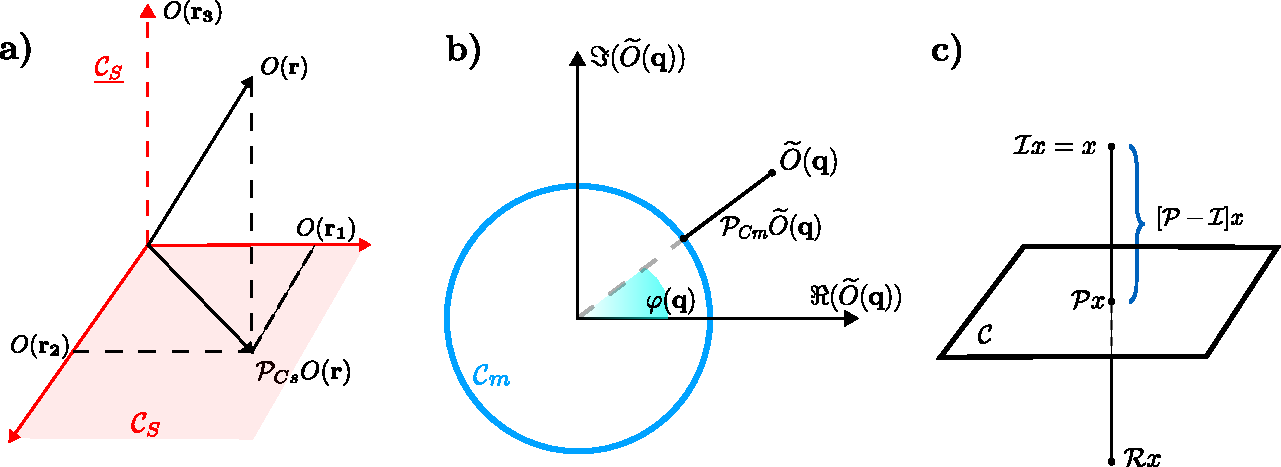
\includegraphics[width=\textwidth]{figures/Intro/projections.pdf}
    \caption{\textbf{a} Geometrical representation of the projection of the object onto the support constraint set.  
    \textbf{b} Geometrical representation of the projection of the object onto the Fourier modulus constraint set.
    \textbf{c} Geometrical representation of the identity, projector and reflector operators. Inspired by \cite{marchesini_unified_2007}}
    \label{fig:projections}
\end{figure}

In our case we have that the projector onto $C_s$ applied to the object sets to zero the values outside the support and does not 
alter the values inside: 
\begin{equation}
    \mathcal{P}_{Cs}(O(\mathbf{r})) = 
    \begin{cases}
        O(\mathbf{r}), & \mathbf{r} \in \mathcal{S} \\
        0,  &  \mathbf{r} \notin \mathcal{S}
     \end{cases}
\end{equation}

On the other hand the projector onto $C_m$ applied to the object replaces the modulus of its Fourier transform with the 
squared root of the measured intensity $m = \sqrt{I(\mathbf{q})}$. 
\begin{equation}
    \mathcal{P}_{Cm}(\widetilde{O}(\mathbf{q})) = \mathcal{P}_{Cm}(A(q)e^{i\varphi(q)}) = \sqrt{I(\mathbf{q})}e^{i\varphi(q)}
    \label{eq:modulus_projection}
\end{equation}

This step forces the modulus of the Fourier transform of the object at the iteration $k$ to be exactly the measured magnitude.  

Since $\mathcal{P}_{Cm}$ and $\mathcal{P}_{Cs}$ operate in two conjugate spaces (direct-reciprocal), when used in sequence 
a direct or inverse Fourier transform is implied in between. The symbol will be omitted to simplify the notation. 

At this point we have all the necessary ingredients to introduce the three main AP algorithms used for BCDI PR. 

\subsection{Error Reduction (ER)}

If we consider as a starting point the object $O^0(\mathbf{r}) = \mathcal{F}^{-1}\{ \sqrt{I(\mathbf{q})}e^{i\varphi^0(\mathbf{q})}\}$, obtained by 
the inverse Fourier transform of the squared root of the measured intensity with a random complex phase array $\varphi^0(\mathbf{q})$, 
we can express the object at the $k-th$ iteration of the \textit{Error Reduction} (ER) algorithm as: 

\begin{equation}
    O^{k+1}(\mathbf{r}) = \mathcal{P}_{Cm}\mathcal{P}_{Cs}(O^{k}(\mathbf{r}))
    \label{eq:ER}
\end{equation}

This is the simplest and most intuitive AP algorithm as it only projects back and forth the object between the two sets. 
Although it guarantees linear convergence, ER is not optimal since it only converges to the nearest local minimum, and it is unable 
to escape it. For this reason in typical BCDI it is used to at the end of the PR, when the current estimate is close enough 
to the final solution.
Additionally, one can define the magnitude error functional $\varepsilon_m(O)$ as: 
\begin{equation}
    \varepsilon_m(O) = || \mathcal{P}_{Cm}(O)  - O ||_{L2} 
    \label{eq:error_magnitude}
\end{equation}
i.e. the Euclidean distance between the current estimate $O$ and its projection onto the Fourier modulus constraint set. 
Differentiating this functional with respect to $O$ yields the gradient $\nabla \varepsilon_m(O)$, which points in the 
direction that reduces the Fourier magnitude mismatch, or in other words, the natural descent direction of the error.
If this gradient is further restricted to the support constraint set, one obtains a 
\textit{projected gradient-descent step} $\nabla_s \varepsilon_m(O)$ which is the part of the descent direction that 
lies inside the feasible object region.

Marchesini shows that the ER step can thus be rewritten as:
\begin{equation}
    O^{k+1}(\mathbf{r}) = \mathcal{P}_{Cs}(O^{k}(\mathbf{r})) - \frac{1}{2}\nabla_s \varepsilon^{2}_m(O^{k}(\mathbf{r}))
    \label{eq:ER_gradient}
\end{equation}

which makes explicit the equivalence between ER and steepest descent projected onto the support constraint set, with 
a fixed step size of $1/2$.

\subsection{Hybrid Input-Output (HIO)}
The Hybrid-Input Output (HIO) algorithm introduces a nonlinear feedback that is essential to escape local minima. 
Specifically, we can express the object at the $k-th$ iteration as: 

\begin{equation}
    O^{k+1}(\mathbf{r}) = 
    \begin{cases}
        \mathcal{P}_{Cm}(O^{k}(\mathbf{r})), &   \mathbf{r} \in \mathcal{S} \\
        (\mathcal{I} -\beta\mathcal{P}_{Cm})(O^{k}(\mathbf{r})),  & \mathbf{r} \notin \mathcal{S}
     \end{cases}
     \label{eq:HIO}
\end{equation}

where $\beta$ is a positive hyperparameter with value typically around $0.9$.
Inside the support, the estimate is replaced by its Fourier-modulus projection. Outside the support, instead of being 
set to zero (as in ER), the estimate is updated with a feedback term proportional to the modulus projection. 
This subtraction, which can in principle yield negative values as well, prevents stagnation and allows the algorithm 
to explore solutions that are consistent with both the support and modulus constraints.
However, it is worth mentioning that due to the nonlinear feedback outside the support, HIO does not converge to local 
minima but rather towards \textit{saddle} points of the error functional. For this reason HIO is used in
combination with ER: HIO drives the reconstruction away from traps by oscillating near saddle points, and ER then 
provides stable convergence once the estimate is close to a true solution. 

\begin{figure}[H]
    \centering
    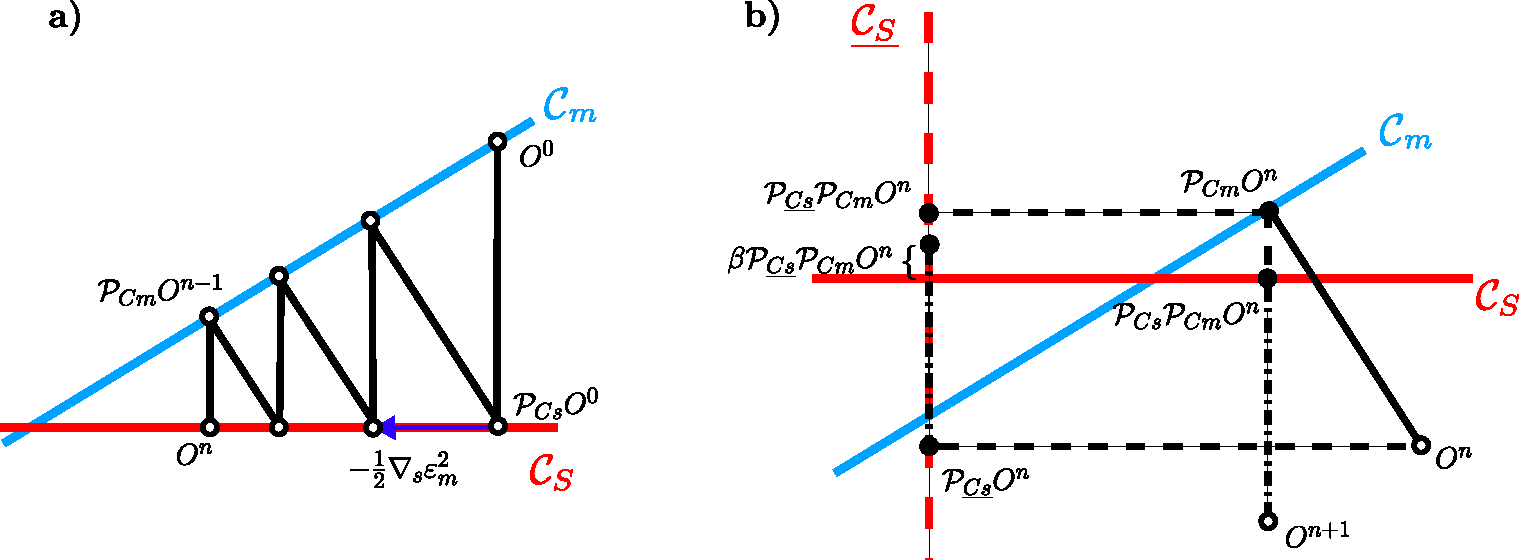
\includegraphics[width=\textwidth]{figures/Intro/ER_HIO.pdf}
    \caption{\textbf{a} Geometrical representation of the ER algorithm. Red and blue lines represent the support and 
    Fourier modulus constraint sets respectively. The alternated projections on the two constraint sets drive eventually 
    the estimate to the intersection. This is however only valid in a local subset of the solution space, where the -
    generally non-convex - modulus constraint set is convex and . 
    \textbf{b} Geometrical representation of the HIO algorithm .
     Inspired by \cite{marchesini_unified_2007}}
    \label{fig:projections}
\end{figure}


\subsection{Relaxed Averaged Alternating Reflections (RAAR)}
Another AP algorithm typically used in CDI is the Relaxed Averaged Alternating Reflections (RAAR) developed by Luke 
in 2004 \cite{Luke_2004}. According to this algorithm the object at the $k-th$ iteration is: 
\begin{equation}
    O^{k+1}(\mathbf{r}) =\beta\frac{1}{2}(\mathcal{R}_{Cs}\mathcal{R}_{Cm} + \mathcal{I})(O^{k}(\mathbf{r})) + (1-\beta)\mathcal{P}_{Cm}(O^{k}(\mathbf{r}))
    \label{eq:RAAR}
\end{equation}

where $\beta \in [0,1]$. 
Eq.\ref{eq:RAAR} can be split into two terms. The first term, known as Average Alternating Reflection (ARR) \cite{AAR_2004} 
acts like an average of the current estimate and its reflection across both constraints sets. The alternated reflections search 
for the intersection of the two sets, which is a fixed point of the problem, while exploring more broadly the solution 
space as they do not project directly on the constraint sets. The second term is a relaxation term that 
projects the current estimate on the modulus set, like in the HIO and ER. 

In short, one could see the RAAR as a controlled (through $\beta$) balance of exploration and stability. 

\subsection{Support update}
At this point of the discussion we should ask ourselves how do we know the \textit{support} function $\mathcal{S}$
required in all PR algorithms? We have said that in the BCDI case we typically do not know the shape of the particle 
a priori, and should therefore come as product of the PR.  
It is common practice in iterative phase retrieval to estimate the initial support 
from the object's autocorrelation,
\begin{equation}
    A(\mathbf{r}) = \mathcal{F}^{-1}\{ I(\mathbf{q}) \}
\end{equation}

However, the autocorrelation extends over a region roughly twice the linear size of the true object (see Fig.). 

An important step forward was introduced by Marchesini in 2003~\cite{Marchesini_shrinkwrap}: 
the \textit{shrinkwrap algorithm}, which adaptively refines the support during reconstruction. 
After a given number of phase retrieval iterations, the modulus of the current object estimate is 
convolved with a Gaussian kernel and subsequently thresholded (typically at $\sim$20\% of the maximum value), 
yielding a binary mask that defines the updated support. 

This adaptive support refinement was shown to significantly improve convergence and reconstruction quality 
in many experimental cases (depending on the signal-to-noise ratio and choice of threshold), and it is now a 
standard component of BCDI phase retrieval pipelines.\\

Later in the text we will refer to ``standard iterative algorithms'' or ``conventional PR'' as the combination of AP 
algorithms and support updates like Shrinkwrap. 

% \section{Gradient descent based methods}

% Up to now, most of the practical cases of PR for CDI rely on AP algorithms because of the limited computing time necessary 
% for the Fourier transforms and the projector/reflectors operators. 
% Another way of approaching the Phase Problem is via the more classical gradient descent methods. 
% In this case the Phase Problem is formulated as a minimization problem in a specific metric.
% For instance in $L_2$ norm metric it can be written as:

% \begin{equation}
%     O^{\ast}(\mathbf{r})
%     = \argmin_{O \in \mathbb{C}^N}
%     \left\| \, \big| \mathcal{F}\{O\} \big| - \sqrt{I} \, \right\|_2^2 .
% \end{equation} 

% According to which it takes the form of a least-square minimization problem. 
 
% \subsection{Steepest descent}

% \subsection{Conjugate Gradient Methods}

% \section{High strain and local minima}

% \section{Conclusions}